\documentclass[12pt,a4paper]{scrartcl}
\usepackage[utf8]{inputenc}
\usepackage{csquotes}
\usepackage[ngerman]{babel}
\usepackage{amsmath}
\usepackage{amsfonts}
\usepackage{amssymb}
\usepackage{graphicx}
\usepackage{float}
\usepackage{microtype}
\usepackage[backend=biber]{biblatex}
\addbibresource{./sources.bib}
\author{Leon Bentrup}
\title{NSA}
\subtitle{Globale Überwaching und Demokratie?}
\begin{document}
\maketitle
\tableofcontents
\newpage
\KOMAoptions{parskip=full}

\section{Vorwort}
Dass Geheimdienste Telefongespräche und Internetverkehr überwachen, hatte ich eigentlich nie bezweifelt. Was das wirklich bedeutet, das wurde mir aber erst vor zwei Jahren bewusst.

Als im Juni 2013 auf einmal eine ganze Ladung an Informationen über geheime Projekte des amerikanischen Geheimdienstes NSA in den Medien auftauchten, als man langsam begriff, dass es sich dabei um etwas richtig Großes handelt, da spürte ich das ungute Gefühl, dass auch bei meinen Recherchen zu dieser GFS immer wieder auftauchte.

Es fühlt sich an, als könnte man den Schlag in die Magengrube der Freiheit spüren, den die totale Überwachung jedes Menschen der Welt darstellt.

Was im Nachhinein auch völlig logisch ist, mich aber trotzdem beunruhigt, ist die Normalität, die innerhalb der Geheimdienste herrscht. Man muss sich klar machen: Analyst, die Berufsbezeichnung für die „modernen Spione“, die die abgefangenen Daten auswerten, ist ein ganz normaler Job. Analysten wechseln Arbeitgeber und haben LinkedIn-Profile mit Lebensläufen.

Manche Dokumente zeigen Geheimdienste eher als Unternehmen, statt als geheime Organisation: Es gibt Newsletter mit „Wusstest du schon?”-Artikeln, die die Mitarbeiter über die Geschichte des ECHELON-Programms aufklären, für das Anwenden neuer Spionage-Techniken bekommen Mitarbeiter „Skillz-Points“. In anderen Worten: Die Digitalisierung der Welt hat „Spion” zu einem Bürojob gemacht.

\section{Edward Snowden}
\begin{figure}
\centering

\includegraphics[width=0.4\textwidth]{images/snowden.jpg}
\caption{Edward Snowden bei seinem Interview mit Greenwald \cite{commons_snowden}}
\end{figure}
Edward Snowden ist die zentrale Persönlichkeit der Enthüllungen. Nach langjähriger Arbeit in verschiedenen Einrichtungen der amerikanischen Regierung sammelte er eigenständig Millionen von Beweisen für geheime Programme der NSA und anderer Geheimdienste, die er dann durch die Medien an die Öffentlichkeit brachte.

\subsection{Lebenslauf}
Edward Snowden wurde am 21. Juni 1983 geboren.
Da seine beiden Eltern für die Regierung arbeiteten, war es für ihn „normal“, das gleiche zu tun.\cite{wiki_snowden}
Nach seiner Schulzeit trat er 2004 der U.S.-Army bei, mit dem Ziel, in Irak zu kämpfen. Als er nach 3 Monaten bei der Armee einen Trainingsunfall hatte, verließ er sie wieder.\cite{wiki_snowden}
Er arbeitete danach für einige nicht-geheime Einrichtungen der Regierung, bis er 2006, beim Besuch einer Jobmesse, von der CIA rekrutiert wurde, wo er unter anderem bei einem internationalen Treffen 2008 in Genf eingesetzt wurde.
\cite{wiki_snowden}

2009 wechselte er zu DELL, er kümmerte sich um die Computersysteme von Regierungskunden, darunter auch Systeme der NSA und CIA. Sein Einkommen in dieser Position betrug etwa 200~000\$ im Jahr.
Schon dort bekam er Einsicht in einige streng geheime Operationen der NSA und sammelte schon einige Dokumente als Beweis.\cite{wiki_snowden}

Seinen endgültigen Beschluss, die Handlungen der NSA und anderer Geheimdienste an die Öffentlichkeit zu bringen, fasste er 2013. In einem Interview sagte Snowden, dass der 12. März 2013 ausschlaggebend für seine Entscheidung gewesen sei. Dort wurde der Director of National Intelligence (nationaler Geheimdienstdirektor) der USA zur Überwachung von Amerikanern befragt, und log die Mitglieder des Kongresses an, obwohl er unter Eid stand.\cite{wiki_snowden}\cite{citizenfour}

Daraufhin gibt Snowden seinen Job bei DELL auf und wechselte zur Dienstleistungsfirma Booz Allen Hamilton, die Personal für die NSA zur Verfügung stellte. Er war im Geheimdienst offiziell als Systemadministrator tätig, und hatte somit uneingeschränkten Zugriff auf alle Akten des Geheimdienstes. Snowden sagte, dass zu seinen Aufgaben aber auch das Überprüfen und Angreifen feindlicher Computersysteme zählte. Seine Position nannte er „Systems Analyst”\cite{citizenfour}

\subsection{Enthüllungen}

\begin{figure}[H]
\centering
\begin{tabular}{lr}
Australien & 15~000 Dokumente \\
Vereinigtes Köngreich & 58~000 Dokumente \\
Department of Defense & 960~000 Dokumente \\
National Security Agency & 1~700~000 Dokumente \\
& \textbf{ca. 2~700~000 Dokumente}
\end{tabular}
\caption{Zahl der von Snowden gesammelten Dokumente \cite{wiki_snowden}}
\end{figure}

Auch wenn Snowden wollte, dass die geheimen Operationen der NSA an die Öffentlichkeit geraten, war er nicht generell gegen Überwachung. Nur solle Überwachung gezielt und auf Verdacht stattfinden, und nicht so massenhaft, wie die NSA es betreibt.\cite{wiki_snowden}\cite{citizenfour}

Da er also wichtige Operationen der Geheimdienste, zum Beispiel die Überwachung von bekannten Terrororganisationen, nicht gefährden wollte, musste er beim Veröffentlichen der gesammelten Dokumente vorsichtig sein. Er sichtete zunächst selbst alles und sortierte Teile aus, die nichts mit der von ihm kritisierten Massenüberwachung zu tun hatten.\cite{wiki_snowden}\cite{citizenfour}

Außerdem veröffentlichte er die Dokumente nicht selbst, sondern übergab sie der Filmemacherin Laura Poitras und dem Journalisten Glenn Greenwald. Sie sollten die Dokumente dann über die Medien an die Öffentlichkeit bringen.\cite{wiki_snowden}\cite{citizenfour}

\begin{figure}[h]
\centering
\begin{minipage}{0.5\textwidth}
	\centering
	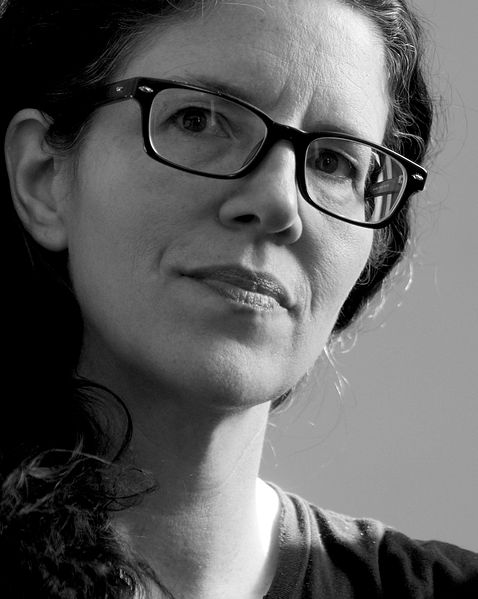
\includegraphics[width=0.7\linewidth]{images/poitras.jpg}
	\captionof{figure}{Laura Poitras \cite{commons_poitras}}
\end{minipage}%
\begin{minipage}{.5\textwidth}
	\centering
	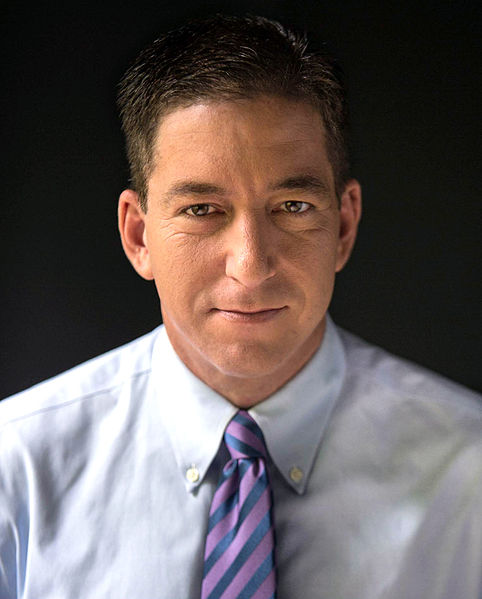
\includegraphics[width=0.7\linewidth]{images/greenwald.jpg}
	\captionof{figure}{Glenn Greenwald \cite{commons_greenwald}}
\end{minipage}
\end{figure}

\subsubsection{Laura Poitras}
Laura Poitras, geboren am 2. Februar 1964 in Boston, ist Produzentin und Filmemacherin. Sie arbeitet seit 2005 an einer Filmreihe über die Welt nach dem 11. September 2001. Nachdem sie den ersten Film der Trilogie veröffentlicht hat, wird sie regelmäßig an der amerikanischen Grenze kontrolliert und befragt. Aus diesem Grund zieht sie nach Berlin um, als sie mit ihrem Film „Citizenfour“ beginnt. Sie befürchtet, dass ihr Filmmaterial beschlagnahmt wird.\cite{praxisfilms}\cite{citizenfour}

\subsubsection{Glenn Greenwald}
Der amerikanische Journalist Glenn Greenwald, der am 6. März 1967 in New York geboren wurde, ist die zweite Person, die Snowden kontaktierte. Er studierte Philosophie und Rechtswissenschaften.\cite{wiki_greenwald} Von 1996 bis 2005 arbeitete er in einer eigenen Anwaltskanzlei, die sich auf Verfassungs- und Bürgerrechte (von US-Bürgern) spezialisierte.\cite{unclaimed_response}

In seinen Blog „Unclaimed Territory“ schrieb Greenwald bis 2007 unter anderem über frühere Affären der NSA, bis er später zum Online-Magazin „salon.com“ und schließlich im Juni 2012 zur britischen Tageszeitung „The Guardian“ wechselte. Im Guardian veröffentlichte Greenwald auch den ersten Artikel über das Snowden-Material.\cite{wiki_greenwald}

2014 gründete er zusammen mit Laura Poitras die Nachrichtenseite „The Intercept“.\cite{intercept_about}

\section{Überwachung}
Aus den von Edward Snowden gesammelten Dokumenten gehen einige Informationen über Programme hervor, die eine massenhafte, globale Überwachung der digitalen Kommunikation ermöglichen.

Heute werden sämtliche Formen der Kommunikation über das Internet abgewickelt. Früher war das Internet noch ein Dienst, der über das Telefonnetz funktionierte, heute ist Telefonie ein Dienst, der über das Internet funktioniert. Der normale Internetverkehr läuft neben Festnetz und Mobilgesprächen, SMS, Fax, Fernsehen, den Bildern von Überwachungskameras und vielem weiteren über ein weltweites Netz von Glasfaserkabeln, die man Internet-Backbone („Rückenmark des Internets“) nennt.

Dies Bedeutet natürlich auch, dass ein Geheimdienst, der Zugriff auf das Internet erhält auch Zugriff auf sämtliche anderen Formen der Kommunikation erhält. Viele Programme der NSA beschäftigen sich aus diesem Grund auch genau damit.

\subsection{XKeyscore}
Die NSA sammelt auf unterschiedlichste Arten Daten: Partnerschaften mit Internetanbietern und Softwarefirmen wie Microsoft oder RSA, das Infiltrieren von Netzwerkhardware, aktivem Hacken von Systemen, Abhören von Funk- und Satellitenkommunikation und so weiter. Eine riesige Datenmenge, die natürlich nicht von Hand analysiert werden kann.

Das XKeyscore-System beschäftigt sich nicht mit dem Sammeln von Daten, sondern mit dem Auswerten von bereits gesammelten Daten. XKeyscore ist auch nicht nur ein einziges System, sondern es gibt mehrere Instanzen, die Nahe am Ort der Datenerfassung lokalisiert sind.\cite{nsa_xkeyscore} Es gibt aber die Möglichkeit eine Suchanfrage an alle XKeyscore-Systeme der Welt zu schicken.\cite{nsa_xksvoip}

\begin{figure}[H]
\centering
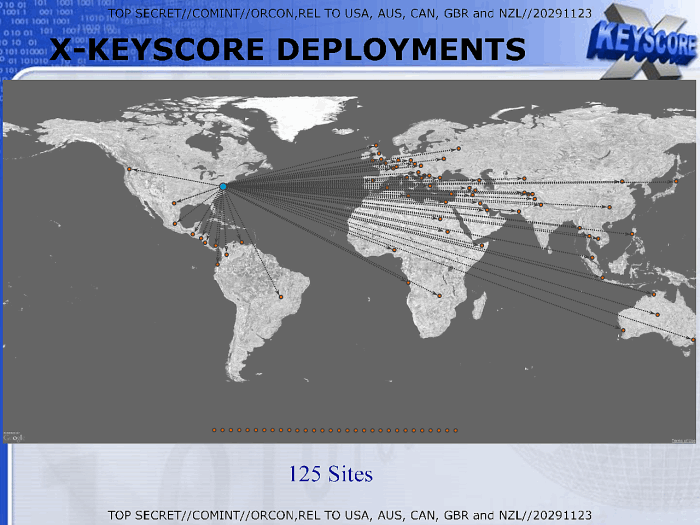
\includegraphics[width=\textwidth]{images/xks_sites.png}
\caption{XKeyscore-Standorte. NSA-Präsentation \cite{nsa_xksdeployments}}
\end{figure}

\paragraph{Datenquellen}
Zunächst werden die Rohdaten von verschiedenen anderen NSA-Projekten und von Geheimdienstpartnern gesammelt. Von folgenden NSA-Operationen ist bekannt, dass sie als Quelle für XKeyscore dienen:

\begin{itemize}
\item \textbf{SCS} (Special Collection Service), Gezieltes Abhören, z.B. in Botschaften durch das Anbringen „klassischer“ Spionagewerkzeuge (Wanzen, Kameras, Telefonleitung anzapfen, etc.)\cite{nsa_scs} Zu diesem Projekt gehörte auch das Abhören des Handys von Angela Merkel.\cite{golem_scs}

\item \textbf{SSO} (Special Sources Operations), Kooperationen mit Internetanbietern, um direkten Zugriff auf deren Netzwerk zu erhalten. Dies geschieht entweder im Einverständnis des Anbieters, der dafür auch bezahlt wird, oder durch richterlichen Beschluss.\cite{nsa_sso}

\item \textbf{ECHELON} (auch FORNSAT genannt), das Abhören von Satelliten und Funksignalen durch eine Vielzahl an Bodenstationen.\cite{eu_echelon} Auch die Bad Aibling Station in Bayern mit ihren vielen Antennen und Radomen zählte bis zu ihrer Übernahme durch den BND zu ECHELON.\cite{eu_echelon}

\item \textbf{TAO} (Tailored Access Operations), Infiltrieren von Kommunikationssystemen. Die NSA hat eigene Software in Netzwerkequipment (z.B. Router) eingeschleust, mit denen sie Daten abhören, oder sogar eigene Daten in ein Netzwerk einschleusen und damit angeschlossene Geräte „hacken“ können.\cite{schneier_tao}

\item \textbf{Overhead}, mehrere Spionagedrohnen, Satelliten und Flugzeuge hören Funkverbindungen ab, die ebenfalls in XKeyscore eingespeist werden.\cite{wiki_xkeyscore}
\end{itemize}
\cite{nsa_xkssources}

\paragraph{Indexieren der Daten}
Die antreffenden Rohdaten werden dann von einem Verbund aus mehreren leistungsfähigen Linux-Servern verarbeitet. Dabei wird zuerst unwichtiges herausgefiltert, z.B. Internetverkehr von Videoportalen.\cite{gchq_tempora} Die restlichen Daten werden je nach Art von verschiedenen Plug-ins „indexiert“. So gibt es Plug-ins für E-Mails, Webseitenaufrufe oder Telefongespräche, die die Metadaten der Verbindungen (in XKeyscore „Sessions“ genannt) extrahieren und speichern.\cite{nsa_xksguide}\cite{nsa_xkeyscore}

\paragraph{Speicherung}
Wie lange die gesammelten Daten gespeichert werden ist nicht bei jeder XKeyscore-Instanz gleich. Je nach untersuchter Datenmenge und Kapazität der Instanz wird der gesamte Internetverkehr mit Inhalt der Verbindungen für kurze Zeit (2-4 Tage) gespeichert, die Metadaten der Verbindungen sind etwa 30 bis 90 Tage lang abrufbar.\cite{nsa_xkeyscore}

\paragraph{Durchsuchen der Daten}
Über eine Weboberfläche steht berechtigten NSA-Mitarbeitern (Analysten) ein Suchformular zur Verfügung, über das sie auf die riesigen gesammelten Datenmengen zugreifen können.

In einer internen Präsentation der NSA finden sich folgende Beispiele für Suchanfragen, die mittels XKeyscore möglich sind:

\begin{itemize}
\item „Zeige mir Personen, die eine für die Region unübliche Sprache verwenden.“
\item „Zeige mir alle verschlüsselten Word-Dokumente im Iran.“
\item „Zeige mir alle mit PGP verschlüsselten E-Mails im Iran.“
\item „Zeige den Ursprung eines Dokuments.“
\item „Zeige mir alle von der NSA hackbaren Computer im Land X.“
\end{itemize}
(Übersetzt nach \cite{nsa_xkeyscore})

\subsection{Five Eyes}
Die NSA ging mit einigen anderen Geheimdiensten Partnerschaften ein. Darunter zählte auch der Deutsche Bundesnachrichtendienst.\cite{zeit_partner} Die „wichtigsten“ Partner waren allerdings:
\begin{itemize}
\item \textbf{GCHQ}, Government Communications Headquarters, \emph{Vereinigtes Königreich}
\item \textbf{DSD}, Defense Signals Directorate, \emph{Australien}
\item \textbf{CSEC}, Communications Security Establishment Canada, \emph{Kanada}
\item \textbf{GCSB}, Government Communications Security Bureau, \emph{Neuseeland}
\end{itemize}\cite{wiki_ukusa}

Zusammen mit der NSA selbst, nennen sich diese Geheimdienste die „Five Eyes”.\cite{wiki_ukusa}
Das Abkommen zwischen den Five Eyes beinhaltete eine „No-Spy-Vereinbarung”, die Partner haben sich also gegenseitig nicht abgehört, es gab allerdings auch Außnahmen von dieser Regel. Außerdem teilten die Bündnispartner sämtliche gesammelten Daten und entwickelte Technologien.\cite{wiki_ukusa} So hatten alle Geheimdienste der Five Eyes Zugriff auf NSA-Programme wie XKeyscore oder PRISM.\cite{wiki_ukusa}

\subsubsection{Umgehung von Beschränkungen durch die Verfassung}
Das Five Eyes-Bündnis wurde auch genutzt um verfassungsrechtliche Beschränkungen zu umgehen. So darf das GCHQ zum Beispiel nach der Verfassung des Vereinigten Königreichs keinen britischen Staatsbürger abhören. Der amerikanische Geheimdienst NSA, der dies natürlich darf, hört dann für das GCHQ deren Ziel ab und gibt die gesammelten Daten an es weiter.\cite{guardian_intentionalspy}

\subsection{TEMPORA}
Zu den Technologien, die die Five Eyes untereinander weitergeben, gehört auch das Projekt des britischen GCHQ, „Tempora“. Hinter Tempora verbirgt sich eine Instanz des amerikanischen XKeyscore-Systems.\cite{gchq_tempora}

Tempora ist das mit Abstand größte XKeyscore-System. Mehr als 1000 Server an mehr als 3 Standorten ermöglichen das Mitschneiden der Kommunikation über Glasfaserkabel.\cite{gchq_tempora}

Großbritanniens geografische Lage ist für dieses Unternehmen sehr vorteilhaft. In Europa liegt es am nächsten zur amerikanischen Ostküste. Deshalb verlaufen fast alle Untersee-Glasfaserkabel zwischen Europa und Amerika durch Großbritannien. Über diese Glasfaserkabel werden alle Internet- und Telefonverbindungen zwischen den Kontinenten übertragen.\cite{gchq_tempora}

Der GCHQ verschafft sich durch Abkommen mit den Betreibern der Internetknoten Zugang zu diesen Kabeln, und ist somit in der Lage 460 GBit/s\cite{gchq_tempora} (Das 46 Millionenfache der durchschnittlichen Internetgeschwindigkeit in Deutschland\cite{statista_internet}) an Daten in Echtzeit zu sammeln, zu sortieren und zu speichern. Die gesamte Kommunikation, mit Inhalt der Verbindungen werden für 3 Werktage gespeichert. Deshalb nennt der GCHQ das System auch einen „Internet Buffer”, einen Zwischenspeicher für das Internet, der die globale Kommunikation „verlangsamt” und im Nachhinein durchsuchbar macht.\cite{gchq_tempora} Die Metadaten, also Sender, Empfänger, deren Aufenthaltsort und Informationen über deren Endgeräte, Betreff und Zeitpunkt der Nachrichten werden für 30 Tage gespeichert.\cite{gchq_tempora}

\section{Verhältnis zu Deutschland}
Die NSA nannte Deutschland einen „Partner dritter Klasse“\cite{zeit_partner}. Das bedeutet, dass Deutschland, obwohl es ein Abkommen mit der NSA geschlossen hat, abgehört wird.\cite{zeit_partner} Die NSA sammelt ungefähr so viele Datensätze über Deutschland, wie sie auch über China und Russland sammelt. (Siehe Abbildung~\ref{fig:boundless_informant})

% Boundless Informant
\begin{figure}[H]
\centering
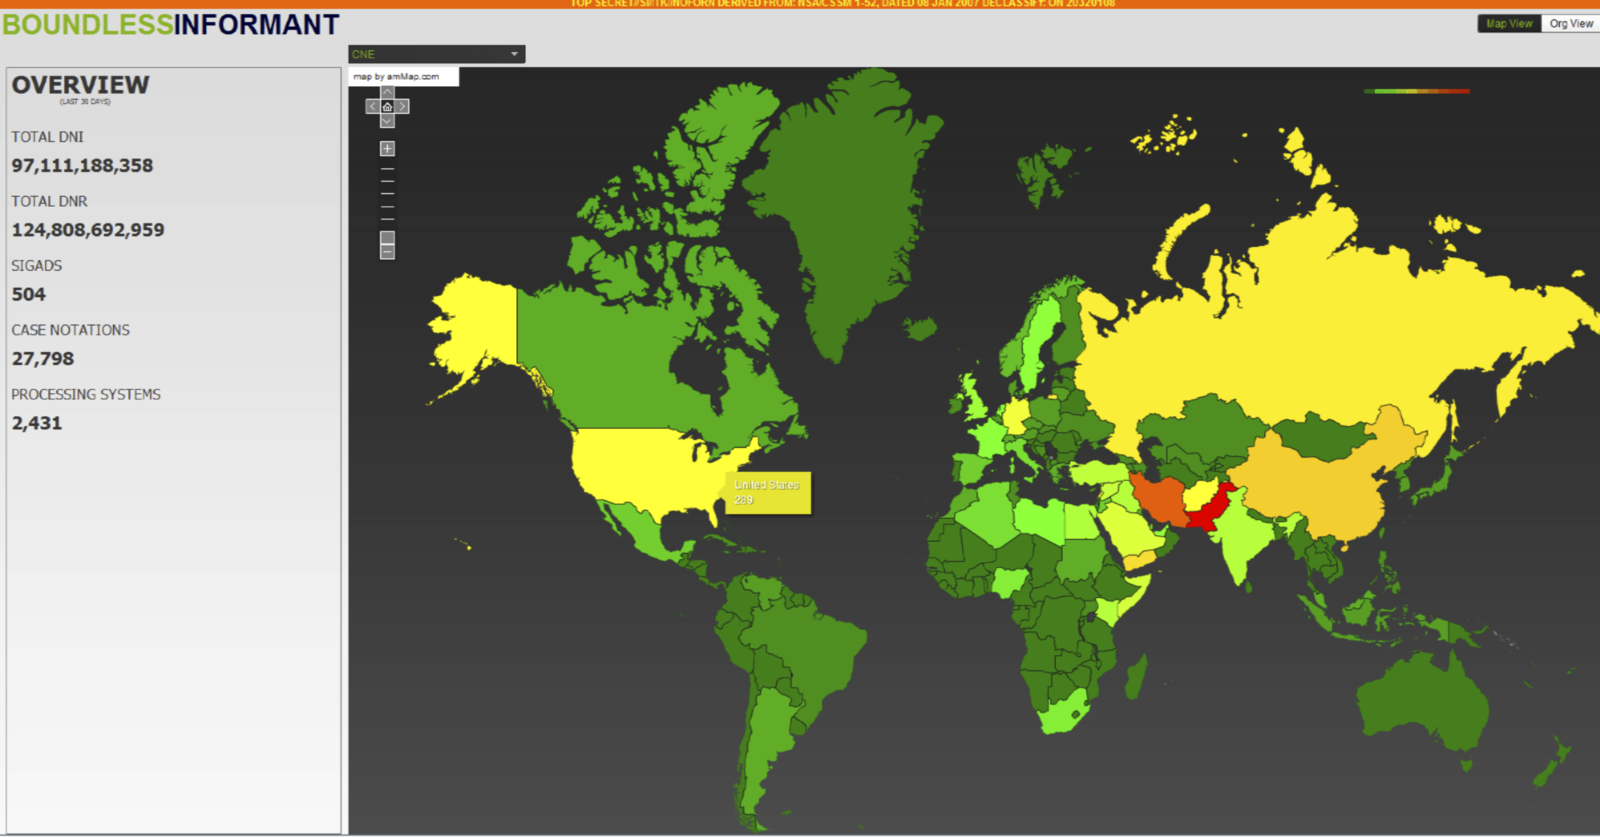
\includegraphics[width=\textwidth]{images/bi.png}
\caption{Übersicht über von der NSA gesammelten Daten nach Land (Boundless Informant)\cite{nsa_bi}}
\label{fig:boundless_informant}
\end{figure}

\subsection{Partnerschaft mit der NSA}
Die Rahmenbedingungen, die die Partnerschaft zwischen Bundesnachrichtendienst, Verfassungsschutz und der NSA kennzeichnen, sind in einem Dokument namens „Terms of Reference“ festgehalten.\cite{zeit_tor}

Die NSA übergibt dem BND das XKeyscore-System, welches dieser dann auf eigenen Servern einsetzen kann. Außerdem darf der BND das System an das Bundesamt für Verfassungsschutz weitergeben. Im Gegenzug gibt Deutschland so viele Daten wie möglich an die NSA weiter, falls diese für deren Ermittlungen relevant sein könnten.\cite{zeit_tor}

\subsection{Operation Eikonal}
Die wohl umstrittenste Operation des BND, die bei den Untersuchungen des NSA-Ausschusses im Bundestag bekannt wurde, ist die „Operation Eikonal“. \cite{zeit_eikonal}

Neben Großbritannien ist auch Deutschland ein wichtiger Standort des Internet-Glasfasernetzes in Europa. In Frankfurt am Main befindet sich der DE-CIX, der am Datendurchsatz gemessen, der größte Internetknoten der Welt ist.\cite{decix_facts}

Zu einigen der vielen Glasfaserleitungen im DE-CIX verschaffte sich der BND Zugang. Er installierte so genannte „Taps“, die den Datenverkehr duplizieren, die Daten werden also zum einen an den Empfänger weitergeleitet, zusätzlich dazu, wird aber eine Kopie der Daten ausgeleitet.\cite{wiki_eikonal} Über eine Standleitung der Telekom wird dann ein Teil der so abgefangenen Daten in den BND-Standort in Pullach weitergeleitet, dort kann er analysiert werden.\cite{zeit_eikonal}

Auf diese Weise können natürlich nicht alle Daten übertragen werden, die am DE-CIX übertragen werden. Die Daten werden deshalb „selektiert”, das heißt, sie werden mit einer Liste von E-Mailaddressen, Telefonnummern, IP-Adressen, Namen und Benutzernamen abgeglichen, und nur relevante Daten werden dann weitergeleitet. Solch eine Liste erhielt der BND auch von der NSA, sie soll etwa 14 Mio. Selektoren enthalten haben.\cite{ard_selektoren}

Darunter waren allerdings auch Selektoren, die deutsche Ziele beinhalteten. Deshalb wurde diese Liste nach BND-Angaben durch ein eigenes Filterungssystem, „Dafis” genannt aussortiert. Dabei wurden z.B. +49-Telefonnummern und E-Mailaddressen die in .de enden aussortiert. Wie die Selektoren wurden auch die Daten, die an die NSA weitergeleitet werden sollten durch dieses System gefiltert.\cite{bundestag_selektoren}

Ob dieses Verfahren rechtmäßig ist, wurde schon von Anfang an bezweifelt, auch von Mitarbeitern des BND selbst. Denn das Dafis-Filtersystem soll nicht einwandfrei funktioniert haben. Man geht von einer Trefferquote von 95\% aus was im Umkehrschluss bedeutet, dass 5\% der Daten von Deutschen nicht vom System erkannt und somit zur NSA weitergeleitet wurden. Dies entspricht etwa 2 Terrabyte „grundrechtswiedriger“ Daten, die die NSA pro Stunden von den Deutschen erhält.\cite{wiki_eikonal} Deshalb wurde die Operation Eikonal angeblich 2008 eingestellt. Vor dem NSA-Untersuchungsausschuss sagte ein BND-Mitarbeiter:

\begin{quote}
Eikonal beinhaltete selektive Erfassung von Ausland-Ausland-Transitverkehr. Zeit nicht vergessen: Afghanistan, Terror-Aufklärung. Da wurden selektiert Daten erfasst und automatisiert weitergeleitet. Genaueres nur nicht-öffentlich. Wir machen die Methodik ja immer noch.\cite{wiki_eikonal}
\end{quote}

Es ist also fraglich, ob Eikonal 2008 wirklich eingestellt wurde.

\section{Geheimdienste in Deutschland}
\begin{quote}
\textbf{Artikel 10, GG} \\ \\
(1) Das Briefgeheimnis sowie das Post- und Fernmeldegeheimnis sind unverletzlich.

(2) Beschränkungen dürfen nur auf Grund eines Gesetzes angeordnet werden. Dient die Beschränkung dem Schutze der freiheitlichen demokratischen Grundordnung oder des Bestandes oder der Sicherung des Bundes oder eines Landes, so kann das Gesetz bestimmen, daß sie dem Betroffenen nicht mitgeteilt wird und daß an die Stelle des Rechtsweges die Nachprüfung durch von der Volksvertretung bestellte Organe und Hilfsorgane tritt.
\end{quote}

Nach dem Grundgesetz ist die private Kommunikation prinzipiell geschützt. Wie in Absatz 2 beschrieben findet aber eine Einschränkung durch das „Gesetz zur Beschränkung des Brief-, Post-, und Fernmeldegeheimnisses“, kurz G-10-Gesetz statt. Dieses Gesetz ermöglicht Polizei und Geheimdiensten bei ihren Ermittlungen Verdächtige abzuhören.

Deutschland verfügt über drei Geheimdienste, jeder mit ganz bestimmten Aufgaben. Die Aufgaben und Befugnisse der Geheimdienste sind jeweils in einem Gesetz geregelt.
\subsection{MAD}
Der Militärische Abschirmdienst ist, wie der Name schon sagt, der Geheimdienst des Militärs. Seine Hauptaufgabe ist es, die Soldaten der Bundeswehr zu überprüfen (beispielsweise ob sie zu einer rechtsextremen Organisation gehören). Deshalb wird der MAD auch „Verfassungsschutz des Militärs“ genannt.\cite{ard_geheimdienste}

Außerdem sichert der MAD Bundeswehreinsätze im Ausland und versorgt die Truppen dort mit Informationen.\cite{ard_geheimdienste}

\subsection{BfV}
Das Bundesamt für Verfassungsschutz ist der Geheimdienst für das Innere. Der Verfassungsschutz hat zwei Aufgaben: Zum einen soll er extremistische oder verfassungsfeindliche Organisationen überwachen und kontrollieren, zum anderen soll er Deutschland vor Spionage durch das Ausland schützen.\cite{ard_geheimdienste}

Der Verfassungsschutz verfügt über etwa 2800 Mitarbeiter. Er untersteht dem Bundesinnenministerium.\cite{ard_geheimdienste}

\subsection{BND}
Der Bundesnachrichtendienst ist für das Ausland zuständig. Er soll Informationen über das Ausland und \emph{im} Ausland sammeln. Damit soll er für politische Entscheidungen relevante Informationen beschaffen und Bedrohungen, beispielsweise durch internationale Terroristen abwehren.\cite{ard_geheimdienste}

Mit etwa 6500 Mitarbeitern ist der BND der größte deutsche Geheimdienst. Er wird durch das Kanzleramt kontrolliert.\cite{ard_geheimdienste}

\section{Fazit}
Edward Snowden hat mit seinen Veröffentlichungen gezeigt, zu was Geheimdienste in der Lage sind. In den USA waren natürlich die Anschläge vom 11. September 2001 ausschlaggebend für die dramatische Stärkung der Geheimdienste. Einige Jahre freier Entwicklung der Geheimdienste ohne strikte staatliche Kontrollen und wir sind im heutigen Stadium angelangt. Ein weltweites, nahezu lückenloses Netz, das so gut wie jeden Menschen erfasst.

Nach den Enthüllungen 2013 ist das Thema in den Fokus der Öffentlichkeit gerückt. Einige Posten sind geräumt worden, so musste General Keith Alexander, Director der NSA, den Geheimdienst verlassen. Es ist aber nicht davon auszugehen, dass sich am eigentlichen Problem, an der Methodik der Geheimdienste, nach der sie so viel wie möglich sammeln, statt gezielt vorzugehen, etwas ändern wird.

Die großen Geheimdienstprogramme werden weiterentwickelt. Und es werden neue dazukommen. Wenn ich mich entscheiden müsste, was wohl als nächstes in den Fokus der Überwacher rücken wird, würde ich sagen: Verschlüsselung. Bereits jetzt hat die NSA einige Fähigkeiten, wenn es darum geht Verschlüsselungssysteme zu umgehen. Sei es die enorme Rechenleistung, die im NSA-Rechenzentrum in Utah vermutet wird oder absichtlich geschwächte Kryptografiestandards. Im US-Kongress wird derzeit diskutiert, ob man Verschlüsselung gesetzlich beschränken sollte, so dass staatliche Ermittlungsbehörden eine „Hintertür“ zur Verfügung haben.

Verschlüsselung ist, wenn sie richtig angewandt wird das einzige Mittel, um sich vor Spionage durch Staaten zu schützen. Das gilt sowohl für jeden einzelnen Bürger, der mit akzeptablem Zeitaufwand einen adäquaten Schutz vor Überwachung erhält, als auch für Staaten an sich. Das ist die zweite Aufgabe, die Geheimdienste haben: Eigene Kommunikation schützen. Diese Aufgabe wird von der NSA überhaupt nicht beachtet. Wenn die NSA Schwachstellen in Kryptosysteme integriert, dann ist dies mehr Überwachung auf Kosten der Sicherheit der eigenen Kommunikation.

Was der NSA-Skandal noch gezeigt hat, ist, wie die Geheimdienste parlamentarische Kontrolle untergraben. Operationen von NSA und BND, die eindeutig gegen das Grundrecht verstoßen werden trotzdem durchgeführt. Der Geheimdienstdirektor der USA und auch deutsche Amtsträger lügen vor dem Parlament.

Die Geheimdienste müssen umdenken. Die verdachtlose Überwachung muss aufhören, stattdessen sollte es eine gezielte Überwachung von Personen geben, die auch wirklich verdächtig sind. Jeder Eingriff in die Privatsphäre eines Menschen, egal ob im Inland oder Ausland muss von einem ordentlichen Gericht genehmigt werden. Das Briefgeheimnis ist ein Menschenrecht. Ich glaube, dass solch eine gezielte Überwachung, die von Menschen und nicht von Computersystemen ausgeführt wird deutlich effektiver ist, und zugleich weniger Eingriffe in die persönliche Freiheit jedes Einzelnen mit sich zieht.

\newpage
\printbibliography
\vspace{2cm}
Hiermit erkläre ich, dass ich die vorliegende Arbeit selbstständig und ohne fremde Hilfe verfasst und keine anderen Hilfsmittel als angegeben verwendet habe. Insbesondere versichere ich, dass ich alle wörtlichen und sinngemäßen Übernahmen aus anderen Werken als solche kenntlich gemacht habe.
\vspace{2cm}
\hrule
\end{document}
